\section{A short introduction to systems biology}
\subsection{Complex systems in biology}
Fundamental problems:
\begin{enumerate}[label={\arabic*)}]
\item We don't have a construction plan!\\
How can we understand a computer by pure observation?
\item The answer of a biological system is often non-linear\\
Example: The dosis of a drug has to be optimized - it might be lethal if it is too high
\item Biological Systems strongly interact with the environment\\
Immune system: Cell-cell interaction may induce killing of cells
\end{enumerate}
Resume: Compared to engineered systems we have to work with less knowledge, less control and a high degree of non-linearity
\subsection*{What are the goals of systems biology?}
\begin{itemize}[label={$-$}]
\item Explain, how biological systems work!
\item Make reliable predictions of biological systems to different external conditions in a controlled fashion
\end{itemize}
\subsection{Static network models}
In biological systems static networks often describe the steady state of a system. There are two different kinds of approaches to network analysis:\\
First, one may ask how a given network actually works, and second, one can try to construct the underlying network structure by analysing the known part of the network.
\subsubsection{Interaction graphs}
Graphs consist of \underline{nodes} (or vertices) and \underline{edges}. Nodes represent the interacting components (molecules, species, subpopulations) and edges their interactions (chemical reactions, competition in evolution).
\subsubsection{Examples of networks}
\begin{enumerate}[label={(\Alph*)}]
\item Directed network
\begin{tikzpicture}
\node [draw,shape=circle,name=p1,minimum size=0.5mm] at (0,0){};
\node [draw,shape=circle,name=p2,minimum size=0.5mm] at (1,0.5){};
\node [draw,shape=circle,name=p3,minimum size=0.5mm] at (1,-0.5){};
\node [draw,shape=circle,name=p4,minimum size=0.5mm] at (2,0){};
\draw[->,shorten <=2pt,shorten >=2pt] (-1,0)--(p1);
\draw[->,shorten <=2pt,shorten >=2pt] (p1)--(p2);
\draw[->,shorten <=2pt,shorten >=2pt] (p1)--(p3);
\draw[->,shorten <=2pt,shorten >=2pt] (p3)--(p2);
\draw[->,shorten <=2pt,shorten >=2pt] (p2)--(1,1.5);
\draw[->,shorten <=2pt,shorten >=2pt] (p3)--(p4);
\draw[->,shorten <=2pt,shorten >=2pt] (p2)--(p4);
\draw[->,shorten <=2pt] (p4)--(3,0);
\end{tikzpicture}
\item Indirected network
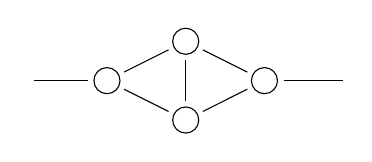
\begin{tikzpicture}
\node [draw,shape=circle,name=p1,minimum size=0.5mm] at (0,0){};
\node [draw,shape=circle,name=p2,minimum size=0.5mm] at (1,0.5){};
\node [draw,shape=circle,name=p3,minimum size=0.5mm] at (1,-0.5){};
\node [draw,shape=circle,name=p4,minimum size=0.5mm] at (2,0){};
\draw[shorten <=2pt,shorten >=2pt] (-1,0)--(p1);
\draw[shorten <=2pt,shorten >=2pt] (p1)--(p2);
\draw[shorten <=2pt,shorten >=2pt] (p1)--(p3);
\draw[shorten <=2pt,shorten >=2pt] (p3)--(p2);
\draw[shorten <=2pt,shorten >=2pt] (p3)--(p4);
\draw[shorten <=2pt,shorten >=2pt] (p2)--(p4);
\draw[shorten <=2pt] (p4)--(3,0);
\end{tikzpicture}
\item Bidirectional network
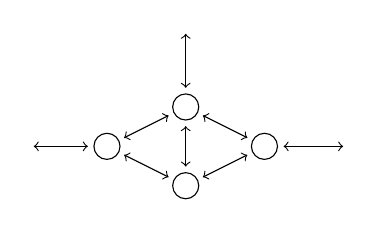
\begin{tikzpicture}
\node [draw,shape=circle,name=p1,minimum size=0.5mm] at (0,0){};
\node [draw,shape=circle,name=p2,minimum size=0.5mm] at (1,0.5){};
\node [draw,shape=circle,name=p3,minimum size=0.5mm] at (1,-0.5){};
\node [draw,shape=circle,name=p4,minimum size=0.5mm] at (2,0){};
\draw[<->,shorten <=2pt,shorten >=2pt] (-1,0)--(p1);
\draw[<->,shorten <=2pt,shorten >=2pt] (p1)--(p2);
\draw[<->,shorten <=2pt,shorten >=2pt] (p1)--(p3);
\draw[<->,shorten <=2pt,shorten >=2pt] (p3)--(p2);
\draw[<->,shorten <=2pt,shorten >=2pt] (p2)--(1,1.5);
\draw[<->,shorten <=2pt,shorten >=2pt] (p3)--(p4);
\draw[<->,shorten <=2pt,shorten >=2pt] (p2)--(p4);
\draw[<->,shorten <=2pt] (p4)--(3,0);
\end{tikzpicture}
\item Signaling network
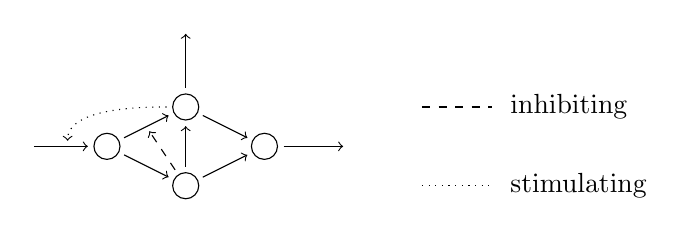
\begin{tikzpicture}
\node [draw,shape=circle,name=p1,minimum size=0.5mm] at (0,0){};
\node [draw,shape=circle,name=p2,minimum size=0.5mm] at (1,0.5){};
\node [draw,shape=circle,name=p3,minimum size=0.5mm] at (1,-0.5){};
\node [draw,shape=circle,name=p4,minimum size=0.5mm] at (2,0){};
\draw[->,shorten <=2pt,shorten >=2pt] (-1,0)--(p1);
\draw[->,shorten <=2pt,shorten >=2pt] (p1)--(p2);
\draw[->,shorten <=2pt,shorten >=2pt] (p1)--(p3);
\draw[->,shorten <=2pt,shorten >=2pt] (p3)--(p2);
\draw[->,shorten <=2pt,shorten >=2pt] (p2)--(1,1.5);
\draw[->,shorten <=2pt,shorten >=2pt] (p3)--(p4);
\draw[->,shorten <=2pt,shorten >=2pt] (p2)--(p4);
\draw[->,shorten <=2pt] (p4)--(3,0);
\draw[->,shorten <=2pt,shorten >=2pt, dashed] (p3)--(0.5,0.25);
\draw[->,shorten <=2pt,shorten >=2pt,dotted] (p2) .. controls +(-0.5,0) and +(0,0.5) .. (-0.5,0);
\draw[dashed,shorten >=3pt] (4,0.5)--(5,0.5);
\draw[dotted,shorten >=3pt] (4,-0.5)--(5,-0.5);
\node [right] at (5,0.5){inhibiting};
\node [right] at (5,-0.5){stimulating};
\end{tikzpicture}
\end{enumerate}
\subsubsection{The properties of graphs}
We represent a biological network with a Graph $\mathcal{G}$ which consits of nodes $N_i$ and edges $e(N_i,N_j)$ connection nodes.
\begin{itemize}[label={}]
\item Degree of a node - $\text{deg}(N_i)=\text{\# of associated edges}$\\
\underline{Example:}\\
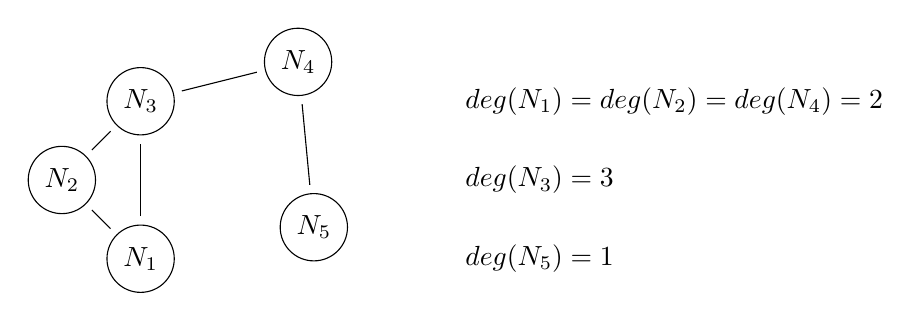
\begin{tikzpicture}[]
\node [draw, shape=circle, name=n1] at (0,0) {$N_1$};
\node [draw, shape=circle, name=n2] at (-1,1) {$N_2$};
\node [draw, shape=circle, name=n3] at (0,2) {$N_3$};
\node [draw, shape=circle, name=n4] at (2,2.5) {$N_4$};
\node [draw, shape=circle, name=n5] at (2.2,0.4) {$N_5$};

\draw [shorten <=3pt, shorten >=3, ] (n1.north) -- (n3.south);
\draw [shorten <= 3pt, shorten >= 3pt] (n1.north west) -- (n2.south east);
\draw [shorten <= 3pt, shorten >= 3pt] (n2.north east) -- (n3.south west);
\draw [shorten <= 3pt, shorten >= 3pt] (n3) -- (n4);
\draw [shorten <= 3pt, shorten >= 3pt] (n4) -- (n5);

\node[right] at (4,2) {$\text{deg}(N_1)=\text{deg}(N_2)=\text{deg}(N_4)=2$};
\node[right] at (4,1) {$\text{deg}(N_3)=3$};
\node[right] at (4,0) {$\text{deg}(N_5)=1$};

\end{tikzpicture}
\end{itemize}
In case of directive graphs it's useful to distinguish between in-degree $\text{deg}_{in}(N_i)$ and out-degree $\text{deg}_{out}(N_i)$ which refer to the number of in- and outgoing edges.\\
The structure of a graph can be represented in an adjacency matrix $A$
\begin{equation*}
A=(a_{ij}) = \begin{cases} 1 & \text{if } e(N_i,N_j) \text{ is an edge in }\mathcal{G}\\ 0 & \text{else}\end{cases}
\end{equation*}
Remark: Undirected edges between nodes $i$ and $j$ are accounted twice, $a_{ij}=a_{ji}=1$\\
\underline{Example:}
\begin{figure}[H]
\begin{multicols}{2}
\begin{center}
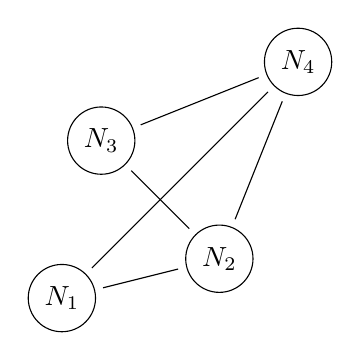
\begin{tikzpicture}
\node [draw,shape=circle,name=n1] at (0,0){$N_1$};
\node [draw,shape=circle,name=n2] at (2,0.5){$N_2$};
\node [draw,shape=circle,name=n3] at (0.5,2){$N_3$};
\node [draw,shape=circle,name=n4] at (3,3){$N_4$};
\draw[shorten <=3pt,shorten >=3pt] (n1)--(n2);
\draw[shorten <=3pt,shorten >=3pt] (n1)--(n4);
\draw[shorten <=3pt,shorten >=3pt] (n2)--(n3);
\draw[shorten <=3pt,shorten >=3pt] (n2)--(n4);
\draw[shorten <=3pt,shorten >=3pt] (n3)--(n4);
\end{tikzpicture}
\end{center}\columnbreak
\begin{center}
\begin{equation*}
A=\begin{pmatrix} 0 & 1 & 0 & 1 \\ 1 & 0 & 1 & 1 \\ 0 & 1 & 0 & 1 \\ 1 & 1 & 1 & 0 \end{pmatrix}
\end{equation*}
\end{center}
\end{multicols}
\end{figure}
\begin{figure}[H]
\begin{multicols}{2}
\begin{center}
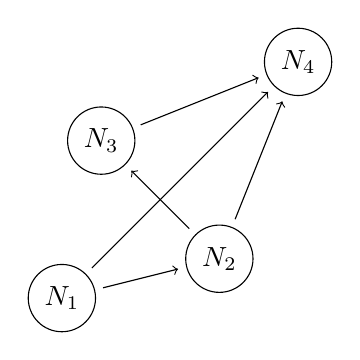
\begin{tikzpicture}
\node [draw,shape=circle,name=n1] at (0,0){$N_1$};
\node [draw,shape=circle,name=n2] at (2,0.5){$N_2$};
\node [draw,shape=circle,name=n3] at (0.5,2){$N_3$};
\node [draw,shape=circle,name=n4] at (3,3){$N_4$};
\draw[->,shorten <=3pt,shorten >=3pt] (n1)--(n2);
\draw[->,shorten <=3pt,shorten >=3pt] (n1)--(n4);
\draw[->,shorten <=3pt,shorten >=3pt] (n2)--(n3);
\draw[->,shorten <=3pt,shorten >=3pt] (n2)--(n4);
\draw[->,shorten <=3pt,shorten >=3pt] (n3)--(n4);
\end{tikzpicture}
\end{center}\columnbreak
\begin{equation*}
A=\begin{pmatrix} 0 & 1 & 0 & 1 \\ 0 & 0 & 1 & 1 \\ 0 & 0 & 0 & 0 \\ 0 & 0 & 1 & 0 \end{pmatrix}
\end{equation*}
\end{multicols}
\end{figure}
\noindent Using the adjacency matrix, some problems in graph theory can be solved with linear algebraic methods\\
E.g.: Which nodes are counted by 2-step paths? This can be obtained from $B=A^2$. In case of the directed graph from above we get:
\begin{equation*}
A^2=\begin{pmatrix} 0 & 1 & 0 & 1 \\ 0 & 0 & 1 & 1 \\ 0 & 0 & 0 & 0 \\ 0 & 0 & 1 & 0 \end{pmatrix}\begin{pmatrix} 0 & 1 & 0 & 1 \\ 0 & 0 & 1 & 1 \\ 0 & 0 & 0 & 0 \\ 0 & 0 & 1 & 0 \end{pmatrix}=\begin{pmatrix} 0 & 0 & 2 & 1 \\ 0 & 0 & 1 & 0 \\ 0 & 0 & 0 & 0 \\ 0 & 0 & 0 & 0 \end{pmatrix}
\end{equation*}
This means there are two 2-step-paths connecting 1\&{}3 and one connecting 1\&{}4 and 2\&{}3. All other pairs of nodes are not connected via two-step-path.
